\chapter{Desenvolvimento do trabalho}

Este capítulo tem como objetivo explicitar quais foram as decisões de projeto que foram tomadas ao longo do desenvolvimento do sistema.

\section{Tecnologias utilizadas}


\subsection{ATmega328P}
Motivação:
Fácil de implementar, ajuda na ideia de open-hardware
Memória programável já dentro do sistema (alguns ATs não têm)
Não é caro (maior parte do custo será nos componentes mecânicos)
Consumo de energia baixo (22mW) em relação à potência proposta (de 1W)

\subsubsection{Análise}


\subsection{Sistema Operacional}
Como o projeto requer controle em tempo real da câmera, é necessário usar um RTOS (real time operating system).
Entre os SOs apresentados, o mais adequado para o controlador Gimbal é o ARM OS.

\subsection{Interface}
SPI (GPIO das placas feitas pela Arduino):
Giroscópio: dados posicionais
Acelerômetro: dados posicionais
Botões (ao menos dois): interface com o usuário
LED (depuração): interface com o usuário
USB:
Carregamento: fazer o código rodar no Arduino 
Depuração: do código na placa

\subsection{Ambiente de desenvolvimento e depuração}
Usaremos as bibliotecas de cada sensor e motor a ser usado, para facilitar a integração
Não há necessidade de sistema de arquivos, já que os dados são tratados ativamente
Usaremos os drivers de interface com o GPIO fornecidos pelo SO
A depuração será feita em cada camada de maneiras diferentes: 
Simulação → aplicação 
QEMU → SO 
LEDs → hardware 

\section{Projeto e implementação}

\subsection{Design}

\begin{figure}[H]
    \centering
    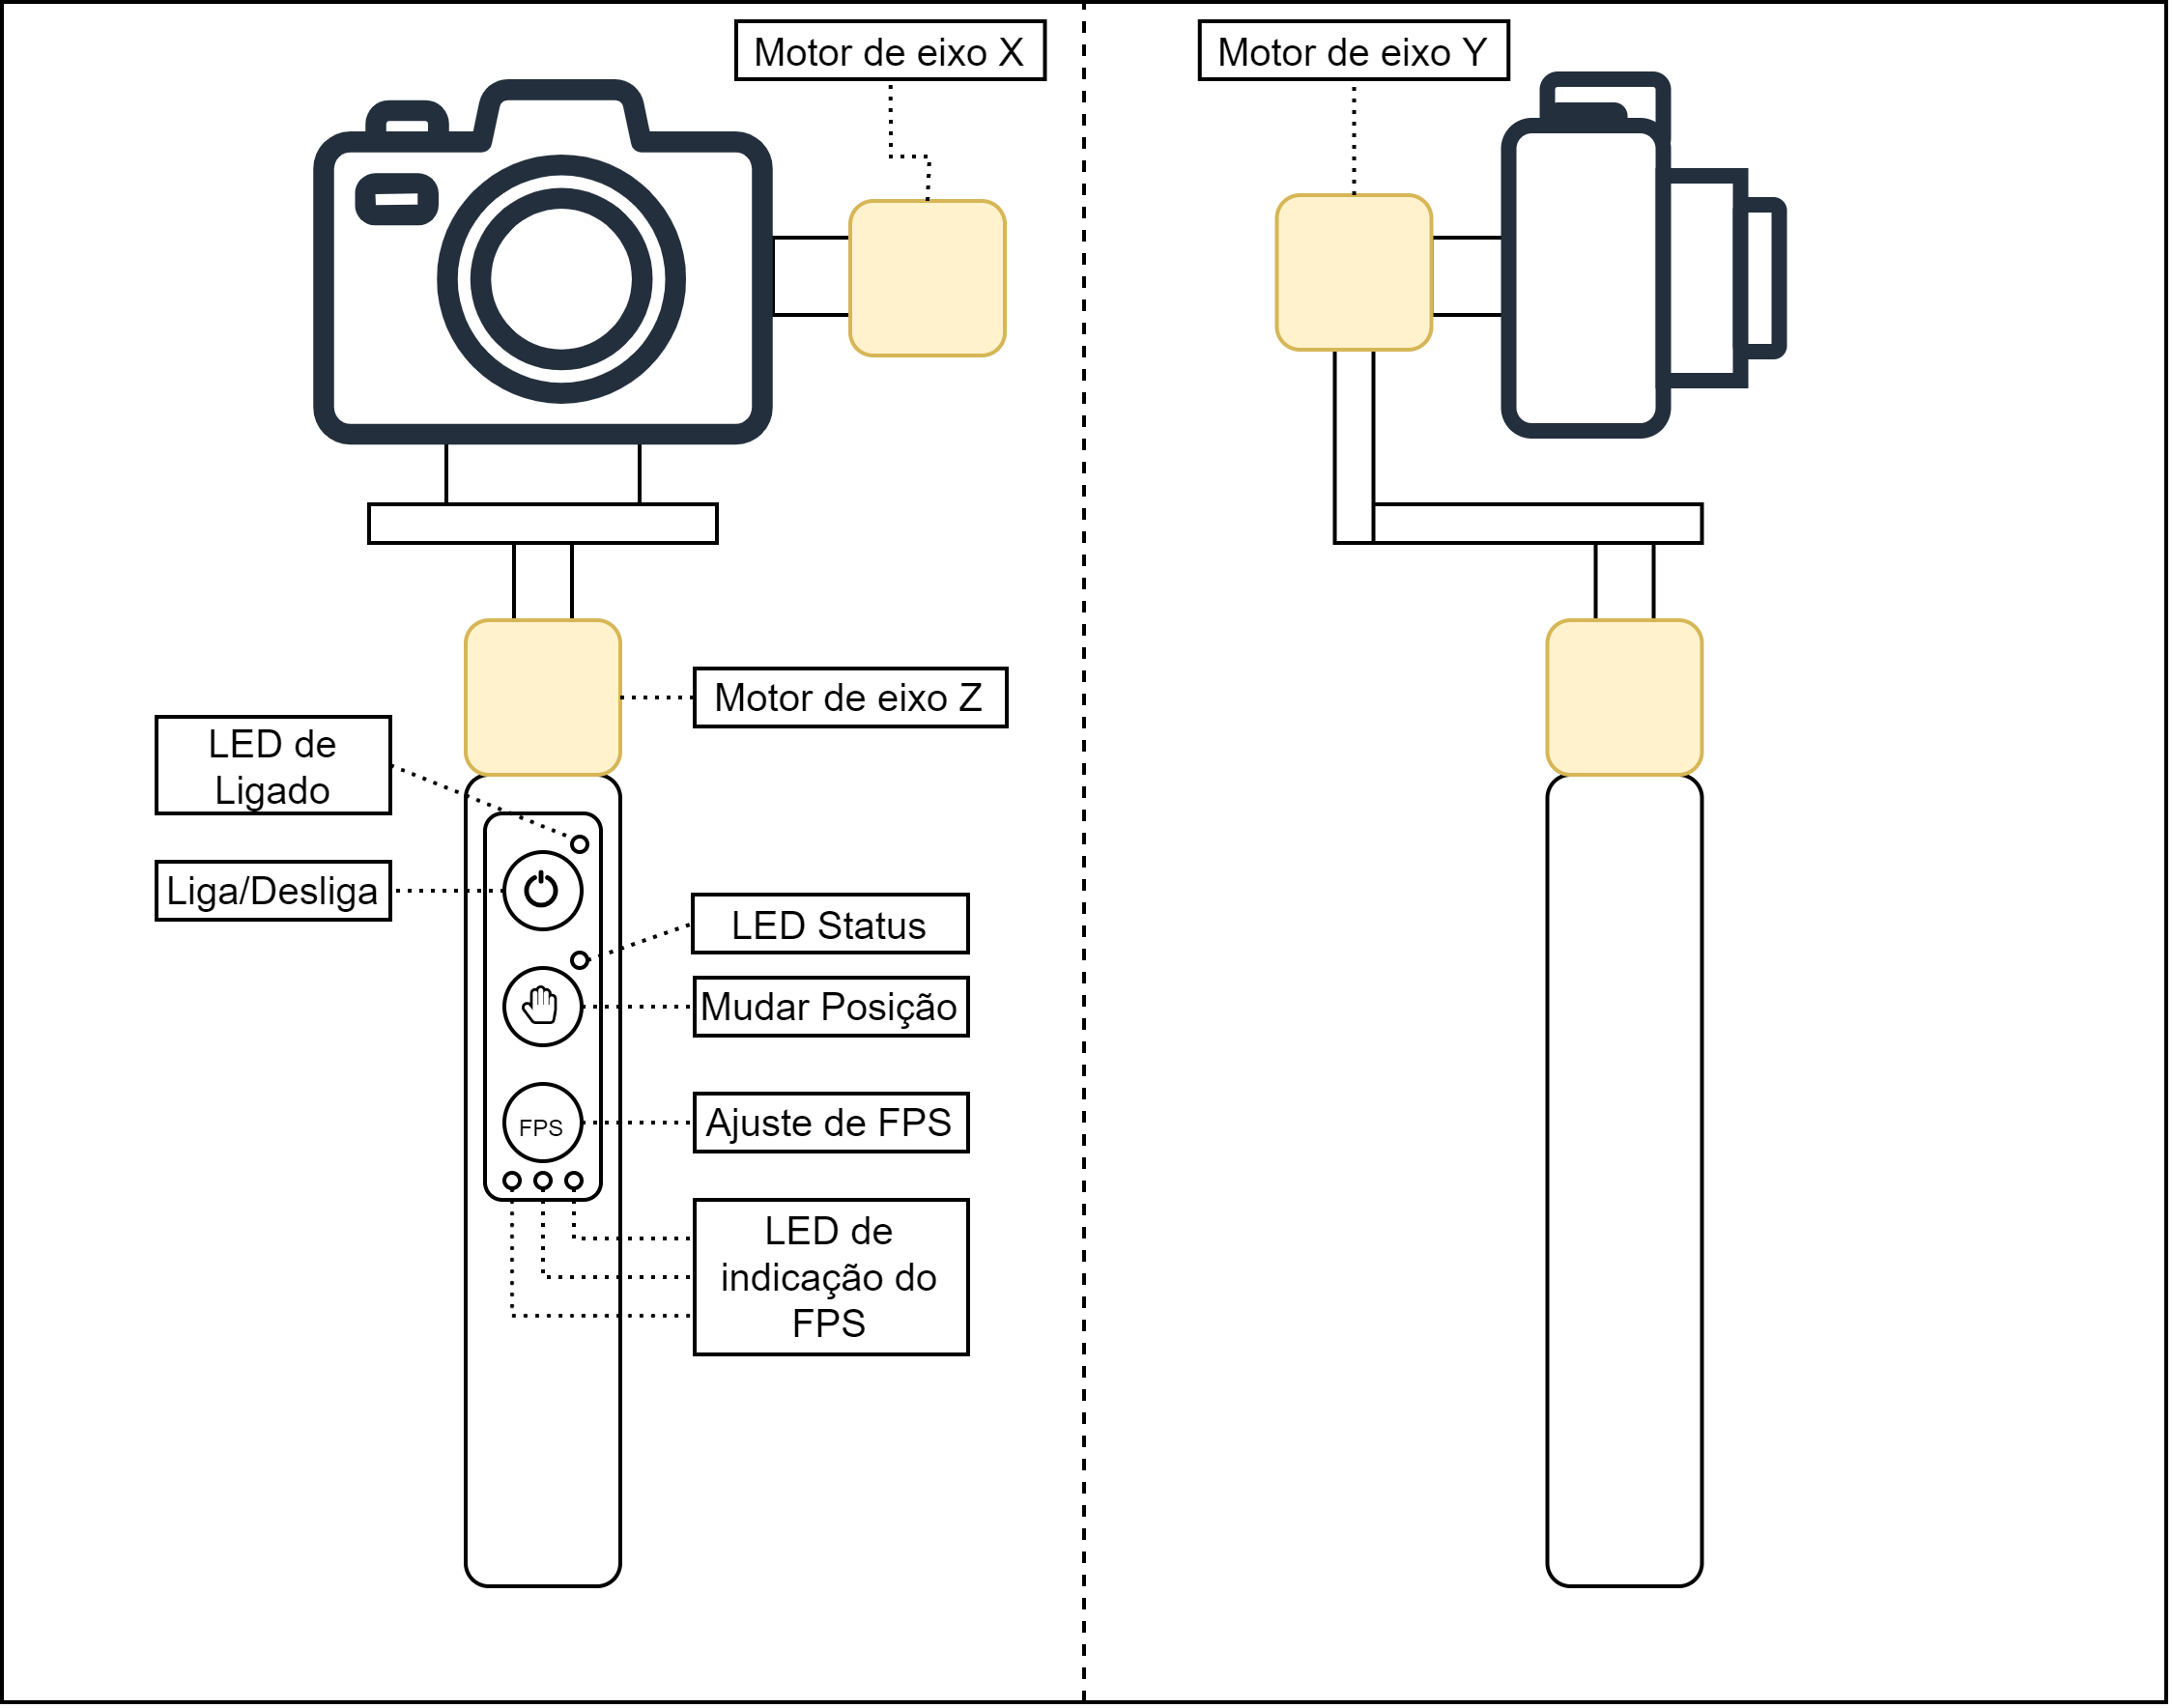
\includegraphics[width=1\textwidth,angle=0]{figures/Design.png}
    \caption{Design básico do projeto}
\end{figure}

\begin{figure}[H]
    \centering
    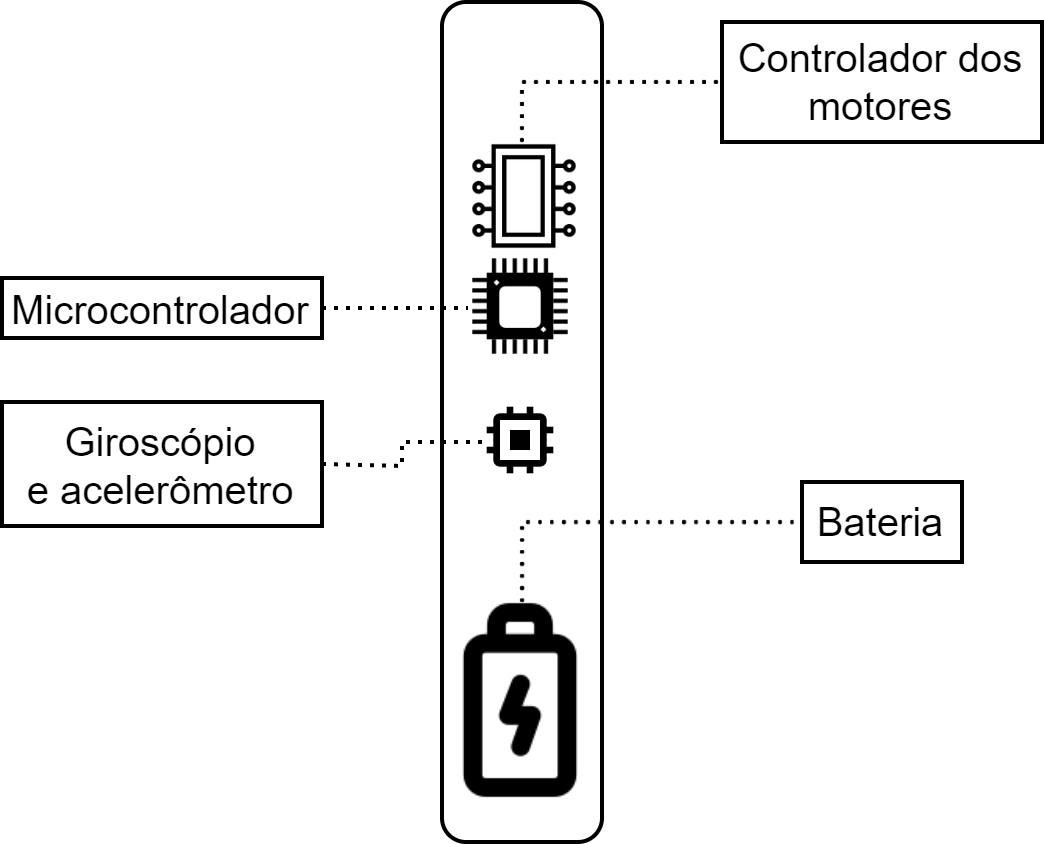
\includegraphics[width=1\textwidth,angle=0]{figures/Design-Page-2.png}
    \caption{Design básico do interior do projeto}
\end{figure}

\section{Testes e avaliação}



